\chapter{Methodology}
\label{chapter:methodology}

\section{Data}

In a first approach we extracted data from the ISIC 2017: Skin Lesion Analysis Towards Melanoma Detection grand challenge datasets \cite{isic2017} which provide a training set with 2000 samples (divided into three classes: 374 melanoma, 254 seborrheic keratosis, and 1372 nevus), a validation set with 150 samples, a test set with 600 samples. However the data was not very good quality and we decided to look for an alternative.

The datasets from the ISIC 2018 grand challenge were largely based on HAM10000\cite{ham10000} which is much more critical. Since the 2018 challenge. Thus we split the 10015 samples ourselves into a training, validation and test set ourselves.

\subsection{Preprocessing}
\label{subsection:preprocessing}

The images in the dataset undergo a number of preprocessing steps.

\begin{enumerate}
    \item Most readily available pretrained models are of network architectures whose input tensor is of square dimensions (e.g. $224 \times 224 \times 3$). Since our dataset's images are of distinct non-square dimensions, it is necessary to resize them to a square. However, resizing them all naively to the network's input tensor dimensions without regards to the image's aspect ratio means that the input fed to the network is of varying distinct aspect ratios which does not constitute a good start. Therefore, the first step is to crop an arbitrarily-sized square of the center of the image which will likely (and, in fact, does) capture the skin lesion.
    \item Resize the images to the target square dimensions. We resize them as soon as possible in the data pipeline in order to reduce the computational costs of any subsequent operations on the images.
    \item Normalize the luminance and apply a 99\% contrast stretch which improves.
\end{enumerate}


\subsection{Augmentation}
\label{subsection:augmentation}

In our binary classification task (melanoma vs non-melanoma) the $m$ samples in the training set are highly imbalanced:

\begin{itemize}
    \item the majority class $S_{maj}$ constitutes 89\% of the samples;
    \item the minority class $S_{min}$ constitutes 11\% of the samples.
\end{itemize}

The number of training samples $m = 2000$ is not enough in proportion to the orders of magnitude of the number of parameters of our networks. We want to augment the data to a new total number of samples $m' \approx 8000$.

With class imbalance in mind, we want the majority class to have a different number of samples $a'$ such that $a' + b' \approx m'$, i.e. $a' \approx b' \approx \frac{m'}{2}$.

That means we must augment the minority class by a factor (i.e. number of transformations applied to each original sample) of $\frac{\frac{m'}{2}}{|S_{min}}$ and the majority class by a factor of $\frac{\frac{m'}{2}}{|S_{maj}}$.

We consider a set $T$ of transformations:

\begin{itemize}
    \item Horizontal flip
    \item Vertical flip
    \item 90º rotation
    \item 180º rotation
    \item 270º rotation
\end{itemize}

We did not consider transformations that change the color (e.g. contrast change, channel shift) or size (e.g. zoom) of features because it would unjustifiably allow the network to incorrectly learn from these misrepresented features. We did not verify this experimentally but it is a very reasonable heuristic because it would also interfere with an expert human diagnosis.

The available augmentations are all k-combinations of the set $T$ for $k \in \{1, ..., |T|\}$, in other words all the possible ways in which you can combine the transformations from the set $T$.

% TODO: rethink this
Affine transformations are not commutative under composition. Applying some transform $T_1$ followed by transform $T_2$ is in general different from applying $T_2$ followed by $T_1$, i.e. the order in which we apply the transforms matters.

\section{Experiments}
\label{section:experiments}

In our search for a model for classification of skin lesions as melanoma, we will conduct experiments based on two contrasting approaches.

We are skeptical of transfer learning, thus our overarching goal is to conclude whether transfer learning provides better or faster results when compared to the conventional end-to-end learning approach in which we train a network from scratch. Simultaneously, within the transfer learning experiments, we should observe that extracting features from higher layers of models trained for ImageNet\cite{imagenet} classification is roughly worse than extracting features from lower layers because these provide more relevant features for skin lesion classification.

\subsection{Transfer Learning Experiments}
\label{subsection:transferlearningexperiments}

In our transfer learning approach we take models of VGG16 \cite{vgg16} and InceptionV3\cite{inceptionv3} architectures pre-trained on ImageNet \cite{imagenet} and transfer the weights to a new model based on techniques we introduced in \ref{section:transferlearning}.

\begin{figure}[h]
    \centering
    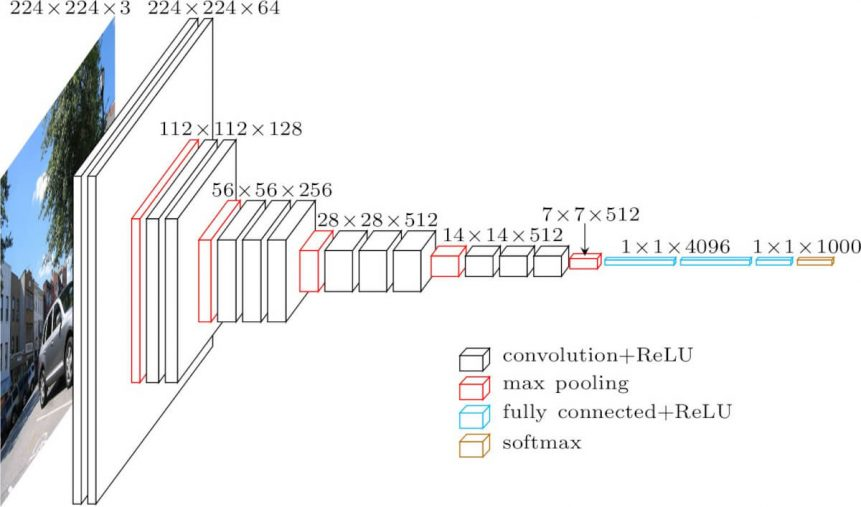
\includegraphics[width=0.5\textwidth]{figs/vgg16.jpg}
    \caption{VGG16 architecture, taken from https://neurohive.io}
    \label{fig:vgg16}
\end{figure}

The basic unit in traditional \ac{CNN} architectures like VGG16 is the convolutional block, which is typically comprised by a number of convolutional layers and a pooling layer at the end to sum up the convolved features. These convolutional blocks are then stacked together in the hope that progressively higher level feature maps are obtained at the end of each block. It is possible that the features at an arbitrary convolutional layer can be used for transfer learning, but in some sense it is expected that the features at a pooling layer are more relevant because that was the intended design. Not only that, but considering features at arbitrary convolutional layers originates a combinatorial explosion of possible feature extractions. As such, we will only extract features at the end of each block (i.e. from pooling layers) because it is heuristically reasonable and significantly reduces the number of layers to extract features from.

In the VGG16 architecture we are interested in extracting $e$ features from $e \in \{18,14,10,6,3\}$ and freezing layers $f \in \{18,14,10,6,3,0\}$. Additionally we grid search the best $\lambda$ for L2-regularization from $\lambda \in \{10^{-10}, ..., 10^{2}\}$ spaced evenly on a log scale.

This originates a rather large number of configurations, so we use a fixed validation scheme (rather than a cross validation scheme) to minimize the computational cost. To ensure the same conditions, we set a fixed seed for every \ac{PRNG}, which in practice means parameters are initialized identically between experiments.

\begin{itemize}
    \item Standardize training and validation samples relative to ImageNet
\end{itemize}

When you're using a pre-trained model based on \ac{CNN}, it is especially important to use a small learning rate because high learning rates increase the risk of losing previous knowledge. Assuming that the pre-trained model has been well trained, which is a fair assumption, keeping a small learning rate will ensure that we don't distort the CNN weights too soon and too much. The whole point of transfer learning is to leverage knowledge from other models, if we use a fast learning rate we risk losing previous knowledge.

\subsection{End-to-End Learning Experiments}

For comparison, in the second set of experiments we design a custom architecture based on reasonable heuristics and train it from scratch.

\begin{figure}[h]
    \centering
    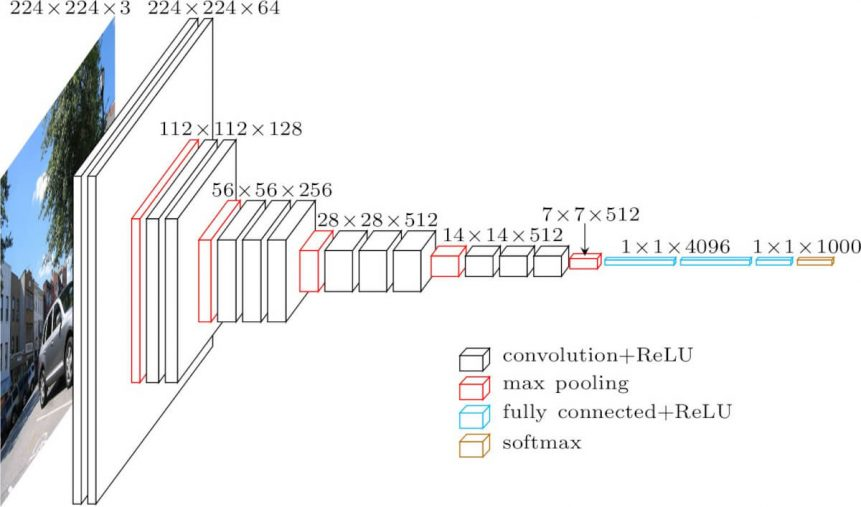
\includegraphics[width=0.5\textwidth]{figs/vgg16.jpg}
    \caption{Custom neural network architecture code-named C1}
    \label{fig:c1}
\end{figure}

\begin{itemize}
    \item Binary cross entropy cost function
    \item Standardize training and validation samples relative to ISIC2018
    \item Weight initialization proposed by He et al \cite{HeWeightInit}
    \item Grid search model selection based on the accuracy on a fixed validation set
    \item Mini-batch (64 samples) \ac{SGD} with an initial learning rate $\eta = 10^{-4}$ that decays by a factor of $10$ if the validation accuracy has not improved significantly in the last $10$ epochs
    \item Train for a maximum of 500 epochs, stopping early if the loss has not changed significantly in the last $30$ epochs
    \item Shuffle the $m$ samples every epoch
    \item Explicit L2 regularization with $\lambda$
\end{itemize}

\section{Evaluation}

Classifiers will be evaluated and compared using F1-score \ref{chapter:binary_classification_metrics}.

\section{Hardware}

Deep learning is very computationally intensive in itself and even more so when we want to run multiple experiments with hyperparameters or even completely different architectures.

\ac{CNN}, the core of most state-of-the-art deep learning applied to computer vision, are computationally complex and embarassingly parallel \cite{chang2017} which the architecture of general purpose \ac{GPU} are appropriate for \cite{gpu} and for which libraries like cuDNN \cite{cudnn} were developed to further leverage the characteristics of \ac{GPU} into even bigger performance improvements.

There is a growing demand for domain-specific hardware designed specifically for the computations necessary in neural network training and inference, like Google's TPU custom ASIC \cite{tpu}, which naturally can achieve major improvements in cost-energy-performance when compared to general purpose hardware like \ac{GPU} that were originally designed for the demands of computer graphics which coincidentally also serve deep learning very well. Nonetheless, \ac{GPU} remain the best cost-effective commodity hardware for this type of computation, especially when not working at the scale of companies like Google and Facebook.

The CPU does little useful computation in a deep learning application where most of the computation is delegated to the GPU.

% TODO: describe machines we used
